\begin{center}
  \textbf{Отчёт лабораторной работы №\envReportLabNumber}
\end{center}

\textbf{Тема}:
<<\envReportTitle>>

\textbf{Цель}:
изучить основы методов Machine Learning в контексте задачи кластерного анализа (cluster analysis),
приобрести навыки работы с методами Machine Learning в системе STATISTICA StatSoft,
осуществить обработку методами Machine Learning индивидуального набора данных и интерпретацию результатов.

% = = = = = = = = = = = = = = = =

\phantomsection
\addcontentsline{toc}{section}{Подготовка к лабораторной работе}

\begin{center}
  \textbf{Подготовка к лабораторной работе}
\end{center}

Для лабораторной работы нужна программа <<Statistica 10>>.
У меня операционная система Ubuntu 22.04.
Statistica 10 под операционную систему WinXP - Win7.
Чтобы запустить на своей операционной системе программу я буду использовать виртуальную машину.

Чтобы установить Windows XP мне нужен диск (ISO-образ).
Microsoft не поддерживает Windows XP в 2022 году.
С сервером Microsoft не скачать Windows XP.
Буду скачивать ISO-образ с торрент \cite{TorrentWinXP}.
Торрент буду скачивать через open source программу qBitTorrent \cite{downloadQBitTorrent}.

В качестве виртуальной машины буду использовать Oracle Virtual Box \cite{downloadVirtualBox}.
Подключаю ISO образ к виртуальной машине и устанавливаю Windows XP.

Statistica 10 прийдется скачать с торрент трекера \cite{downloadStatistica10}.
Нашел не устанавливаемую версию, а portable (переносимую), которая не засоряет систему.
Запускается *.exe файл и все настройки хранятся в папке "STATISTICA 10 RU" рядом с файлом Ststatistica\_10\_ru\_portable.exe. 

Statistica 10 сразу не запуститься, ибо скажет, что не хватает dll.
Скачаем Visual C++ 2008 \cite{downloadVisualCpp2008}.

Для удобства передачи файлов можно использовать либо через почту и мессенджеры в браузере Firefox 52.9.0esr \cite{downloadFirefox5290esr},
либо подключить общий папки (диск Z).

\begin{center}
  \textbf{Пример использования кластерного анализа STATISTICA в автостраховании}
\end{center}

Я в Libre Office Calc \cite{downloadLibreOffice} создал файл
<<cars\_my.xls>> и заполнил данные как в методичке для того, чтобы попробовать сделать так как в методичке по примеру, а затем сделать свой 5-ый вариант.

\lstinputlisting[name=cars_my.csv (cars_my.xls)]
{../sources/cars_my/cars_my.csv}

Удаляю папку <<Statistica 10 RUS>>.

Запускаю Ststatistica\_10\_ru\_portable.exe.

Главная > Открыть > cars\_my.xls > Открыть \\
> Импортировать выбранные лист в Таблицу данных > Sheet1 > OK \\
> Имена переменных из первой строки>Имена наблюдений из первого столбца > OK

Результат смотри на рисунке~\ref{fig:1_1}.

\begin{figure}[!h]
  \centering

  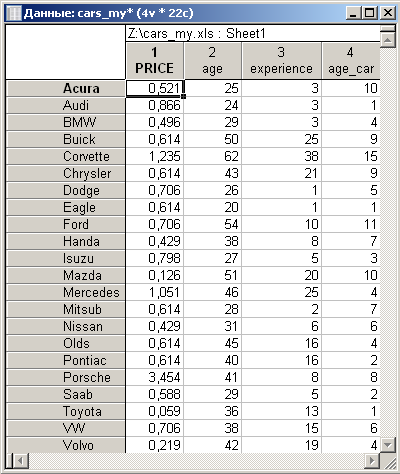
\includegraphics[height=12cm]
  {inc/cars_my/1.1.PNG}

  \caption{Открыли cars\_my.xls в Statistica 10}

  \label{fig:1_1}
\end{figure}

\begin{center}
  \textbf{Масштаб измерений}
\end{center}

Вид > Заголовки переменных > Отображать тип

1 PRICE Вещественный > Формат отображения > Число > Дес. разряды > 3 > OK

2 age Вещественный > Формат отображения > Число > Дес. разряды > 6 > OK

3 experience Вещественный > Тип > Целый > OK > Да

4 age\_car Вещественный > Тип > Целый > OK > Да

Результат смотри на рисунке~\ref{fig:1_2}.

\begin{figure}[!h]
  \centering

  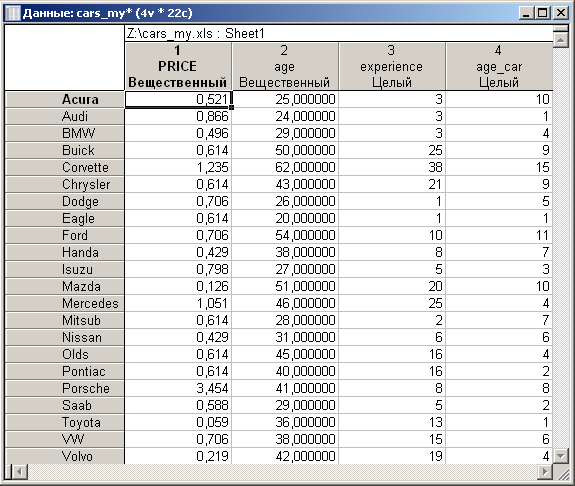
\includegraphics[height=10cm]
  {inc/cars_my/1.2.PNG}

  \caption{Данные}

  \label{fig:1_2}
\end{figure}

\newpage

Данные > Стандартизировать > Переменные > Выбрать все > OK > OK

Результат смотри на рисунке~\ref{fig:1_3}.

\begin{figure}[!h]
  \centering

  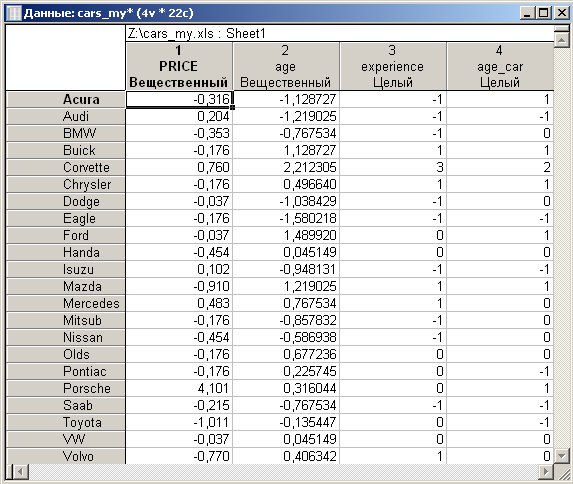
\includegraphics[height=10cm]
  {inc/cars_my/1.3.PNG}

  \caption{Данные}

  \label{fig:1_3}
\end{figure}

Кружок > Сохранить как... > cars\_my\_standartiz.sta > Сохранить

\newpage

\begin{center}
  \textbf{Шаг 1. Иерархическая классификация}
\end{center}

Анализ > Многомерный анализ > Кластерный анализ > Иерархическая классификация > OK \\
> Дополнительно > Переменные > Выбрать все > OK \\
> Объекты > Наблюдения (строки) \\
> Правило объединения > Метод полной связи \\
> Мера близости > Евклидово расстояние \\
> OK > Дополнительно > Вертикальная дендрограмма

Результаты смотри на рисунках~\ref{fig:1_4}, \ref{fig:1_5}, \ref{fig:1_6}.

\begin{figure}[!h]
  \centering
  \begin{minipage}{0.32\textwidth}
    \centering

    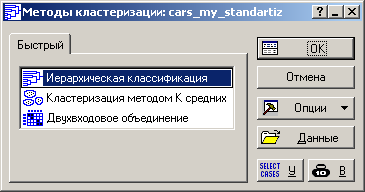
\includegraphics[width=0.99\textwidth]
    {inc/cars_my/1.4.PNG}

    \caption{Окно <<Методы кластеризации>>}
    \label{fig:1_4}
  \end{minipage}
  \begin{minipage}{0.32\textwidth}
    \centering

    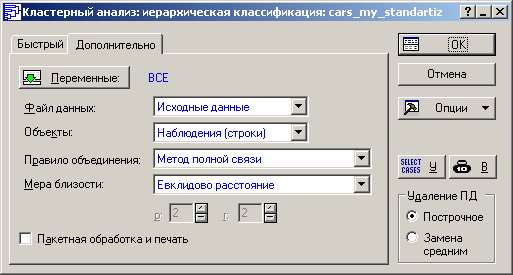
\includegraphics[width=0.99\textwidth]
    {inc/cars_my/1.5.PNG}

    \caption{Окно <<Кластерный анализ>>}
    \label{fig:1_5}
  \end{minipage}
  \begin{minipage}{0.32\textwidth}
    \centering

    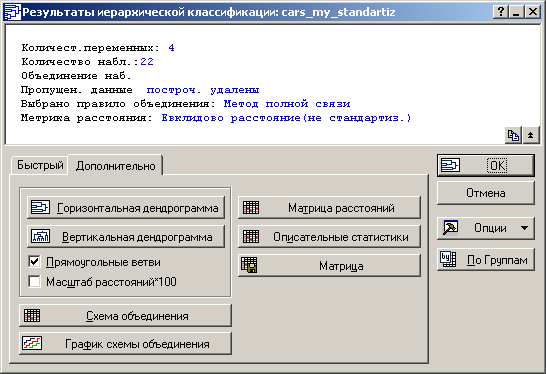
\includegraphics[width=0.99\textwidth]
    {inc/cars_my/1.6.PNG}

    \caption{Окно <<Результаты иерархической классификации>>}
    \label{fig:1_6}
  \end{minipage}
\end{figure}

Результат смотри на рисунке~\ref{fig:1_7}.

\begin{figure}[!h]
  \centering

  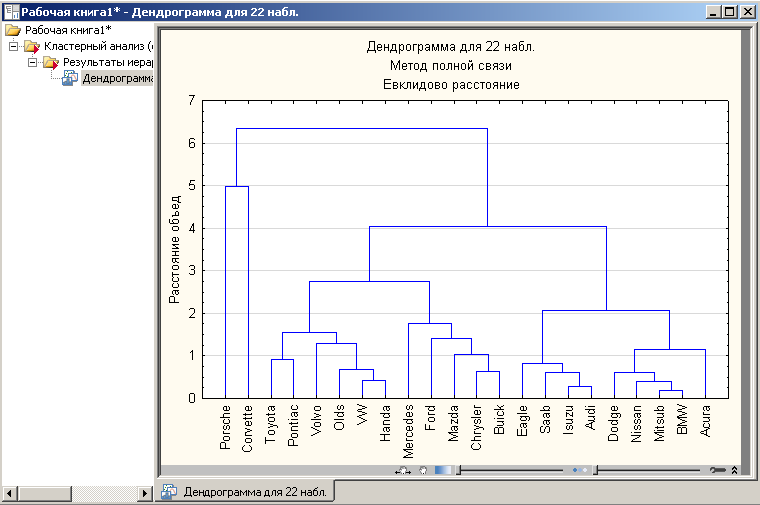
\includegraphics[height=11cm]
  {inc/cars_my/1.7.PNG}

  \caption{Дендрограмма для 22 набл.}
  \label{fig:1_7}
\end{figure}

\newpage

\begin{center}
  \textbf{Шаг 2. Кластеризация методом К средних}
\end{center}

Результата иерархической классификации: cars\_my\_standartiz > Отмена > Отмена \\
> Кластеризация методом К средних > OK \\
> Дополнительно \\
> Переменные > Выбрать все > OK \\
> Объекты > Наблюдения (строки) \\
> Число кластеров > 4 \\
> OK > Дополнительно > Дисперсионный анализ

Результаты смотри на рисунках~\ref{fig:2_1}, \ref{fig:2_2}, \ref{fig:2_3}.

\begin{figure}[!h]
  \centering
  \begin{minipage}{0.49\textwidth}
    \centering

    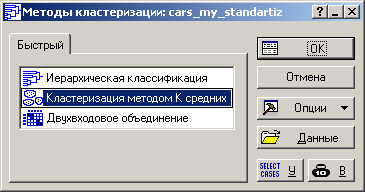
\includegraphics[width=0.99\textwidth]
    {inc/cars_my/2.1.PNG}

    \caption{Окно <<Методы кластеризации>>}
    \label{fig:2_1}
  \end{minipage}
  \begin{minipage}{0.49\textwidth}
    \centering

    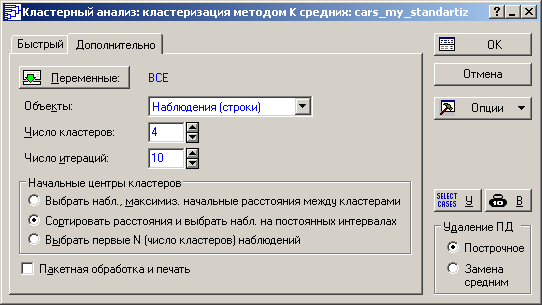
\includegraphics[width=0.99\textwidth]
    {inc/cars_my/2.2.PNG}

    \caption{Окно <<Кластерный анализ>>}
    \label{fig:2_2}
  \end{minipage}
\end{figure}

\begin{figure}[!h]
  \centering

  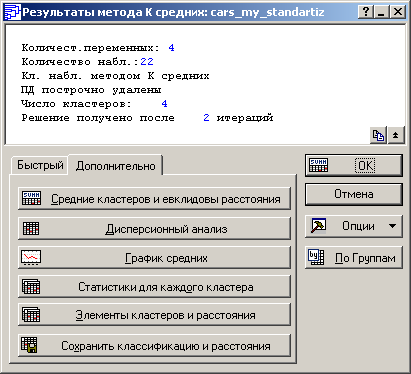
\includegraphics[height=6cm]
  {inc/cars_my/2.3.PNG}

  \caption{Дисперсионный анализ}
  \label{fig:2_3}
\end{figure}

Результаты смотри на рисунке~\ref{fig:2_4}.

\begin{figure}[!h]
  \centering

  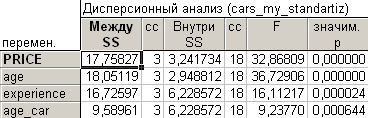
\includegraphics[height=3cm]
  {inc/cars_my/2.4.PNG}

  \caption{Дисперсионный анализ}
  \label{fig:2_4}
\end{figure}

\newpage

Результаты метода К средних: cars\_my\_standartiz > Дополнительно > Элементы кластеров и расстояния

Данные первого кластера смотри на рисунке~\ref{fig:2_5}.

Данные второго кластера смотри на рисунке~\ref{fig:2_6}.

\begin{figure}[!h]
  \centering
  \begin{minipage}{0.49\textwidth}
    \centering

    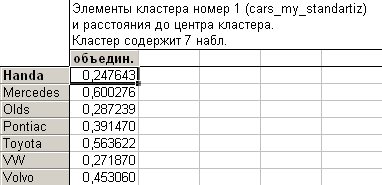
\includegraphics[width=0.99\textwidth]
    {inc/cars_my/2.5.PNG}

    \caption{Первый кластер}
    \label{fig:2_5}
  \end{minipage}
  \begin{minipage}{0.49\textwidth}
    \centering

    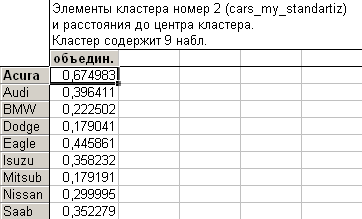
\includegraphics[width=0.99\textwidth]
    {inc/cars_my/2.6.PNG}

    \caption{Второй кластер}
    \label{fig:2_6}
  \end{minipage}
\end{figure}

Данные третьего кластера смотри на рисунке~\ref{fig:2_7}.

Данные четвертого кластера смотри на рисунке~\ref{fig:2_8}.

\begin{figure}[!h]
  \centering
  \begin{minipage}{0.49\textwidth}
    \centering

    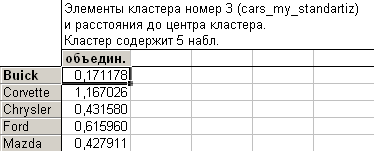
\includegraphics[width=0.99\textwidth]
    {inc/cars_my/2.7.PNG}

    \caption{Третий кластер}
    \label{fig:2_7}
  \end{minipage}
  \begin{minipage}{0.49\textwidth}
    \centering

    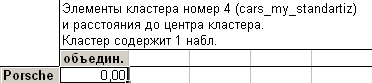
\includegraphics[width=0.99\textwidth]
    {inc/cars_my/2.8.PNG}

    \caption{Четвертый кластер}
    \label{fig:2_8}
  \end{minipage}
\end{figure}

\newpage

\begin{center}
  \textbf{Шаг 3. Кластеризация методом К средних}
\end{center}

Результаты метода К средних: cars\_my\_standartiz > Дополнительно > Сохранить классификацию и расстояние > Выбрать все > OK

Анализ > Основные статистики и таблицы\\
> Группировка и однофакторный ДА > OK\\
> Переменные > 1-PRICE > 6-КЛАСТЕР > OK > OK > Описательные\\
> Статистики > Минимум и максимум > Описательные > Итоговая таблица средних

Результаты смотри на рисунках~\ref{fig:3_1}, \ref{fig:3_2}, \ref{fig:3_3}, \ref{fig:3_4}, \ref{fig:3_5}.

\begin{figure}[!h]
  \centering
  \begin{minipage}{0.49\textwidth}
    \centering

    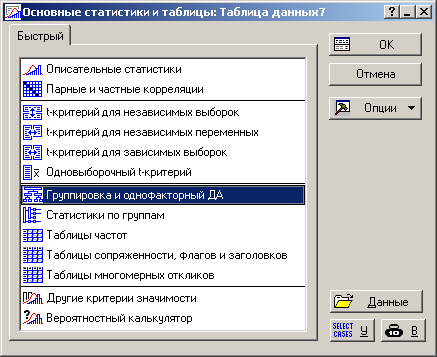
\includegraphics[width=0.99\textwidth]
    {inc/cars_my/3.1.PNG}

    \caption{Окно <<Основные статистики и таблицы>>}
    \label{fig:3_1}
  \end{minipage}
  \begin{minipage}{0.49\textwidth}
    \centering

    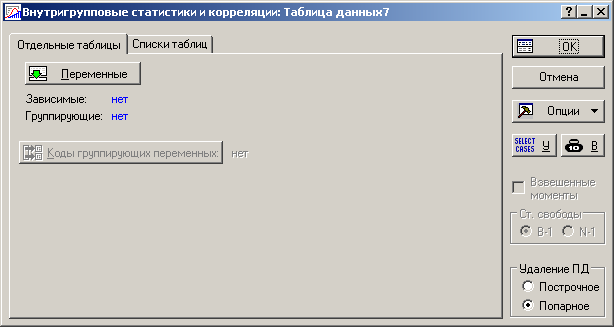
\includegraphics[width=0.99\textwidth]
    {inc/cars_my/3.2.PNG}

    \caption{Окно <<Внутригрупповые статистики и корреляции>>}
    \label{fig:3_2}
  \end{minipage}
\end{figure}

\begin{figure}[!h]
  \centering
  \begin{minipage}{0.49\textwidth}
    \centering

    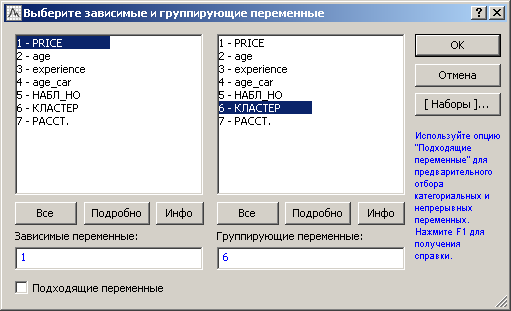
\includegraphics[width=0.99\textwidth]
    {inc/cars_my/3.3.PNG}

    \caption{Окно <<Выберите зависимые и группирующие переменные>>}
    \label{fig:3_3}
  \end{minipage}
  \begin{minipage}{0.49\textwidth}
    \centering

    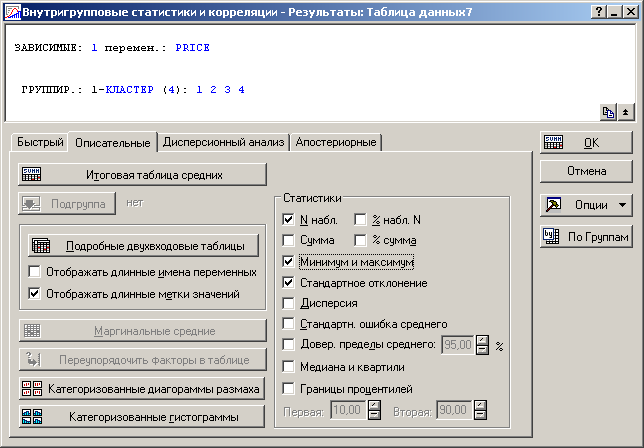
\includegraphics[width=0.99\textwidth]
    {inc/cars_my/3.4.PNG}

    \caption{Окно <<Внутригрупповые статистики и корреляции>>}
    \label{fig:3_4}
  \end{minipage}
\end{figure}

Анализ > Основные статистики и таблицы > Новый\\
> Группировка и однофакторный ДА > OK\\
> Переменные > 2-age > 6-КЛАСТЕР > OK > OK\\
> Описательные > Статистики > Минимум и максимум > Итоговая таблица средних

Результат смотри на рисунке~\ref{fig:3_6}.

\begin{figure}[!h]
  \centering
  \begin{minipage}{0.49\textwidth}
    \centering

    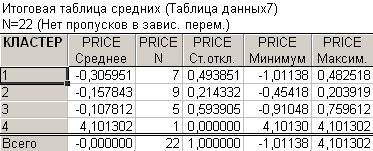
\includegraphics[width=0.99\textwidth]
    {inc/cars_my/3.5.PNG}

    \caption{PRICE}
    \label{fig:3_5}
  \end{minipage}
  \begin{minipage}{0.49\textwidth}
    \centering

    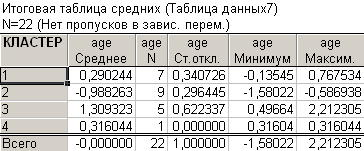
\includegraphics[width=0.99\textwidth]
    {inc/cars_my/3.6.PNG}

    \caption{age}
    \label{fig:3_6}
  \end{minipage}
\end{figure}

Анализ > Основные статистики и таблицы > Новый\\
> Группировка и однофакторный ДА > OK\\
> Переменные > 3-experience > 6-КЛАСТЕР > OK > OK\\
> Описательные > Статистики > Минимум и максимум > Итоговая таблица средних

Результат смотри на рисунке~\ref{fig:3_7}.

Анализ > Основные статистики и таблицы > Новый\\
> Группировка и однофакторный ДА > OK\\
> Переменные > 4-age\_car > 6-КЛАСТЕР > OK > OK\\
> Описательные > Статистики > Минимум и максимум > Итоговая таблица средних

Результат смотри на рисунке~\ref{fig:3_8}.

\begin{figure}[!h]
  \centering
  \begin{minipage}{0.49\textwidth}
    \centering

    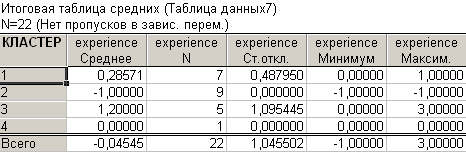
\includegraphics[width=0.99\textwidth]
    {inc/cars_my/3.7.PNG}

    \caption{experience}
    \label{fig:3_7}
  \end{minipage}
  \begin{minipage}{0.49\textwidth}
    \centering

    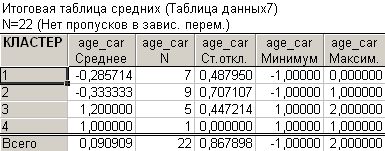
\includegraphics[width=0.99\textwidth]
    {inc/cars_my/3.8.PNG}

    \caption{age\_car}
    \label{fig:3_8}
  \end{minipage}
\end{figure}

Анализ > Основные статистики и таблицы > Новый\\
> Группировка и однофакторный ДА > OK\\
> Переменные > (1-PRICE, 2-age, 3-experience, 4-age\_car) > 6-КЛАСТЕР > OK > OK\\
> Быстрый > Графики взаимодействий. Результаты смотри на рисунках~\ref{fig:3_9}, \ref{fig:3_10}, \ref{fig:3_11}, \ref{fig:3_12}, \ref{fig:3_13}, \ref{fig:3_14}.

\begin{figure}[!h]
  \centering
  \begin{minipage}{0.49\textwidth}
    \centering

    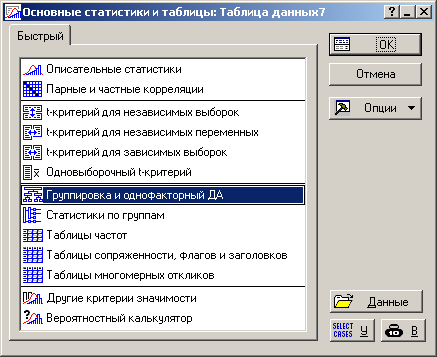
\includegraphics[height=5cm]
    {inc/cars_my/3.9.PNG}

    \caption{Окно <<Основные статистики и таблицы>>}
    \label{fig:3_9}
  \end{minipage}
  \begin{minipage}{0.49\textwidth}
    \centering

    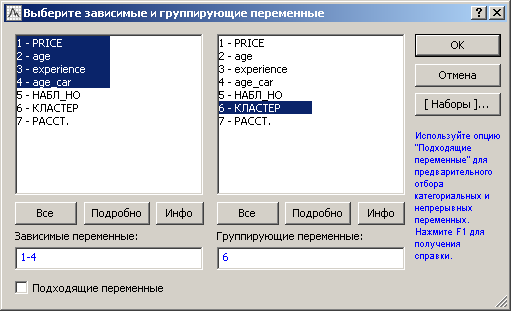
\includegraphics[height=5cm]
    {inc/cars_my/3.10.PNG}

    \caption{Окно <<Выберите зависимые и группирующие переменные>>}
    \label{fig:3_10}
  \end{minipage}
\end{figure}

\begin{figure}[!ph]
  \centering

  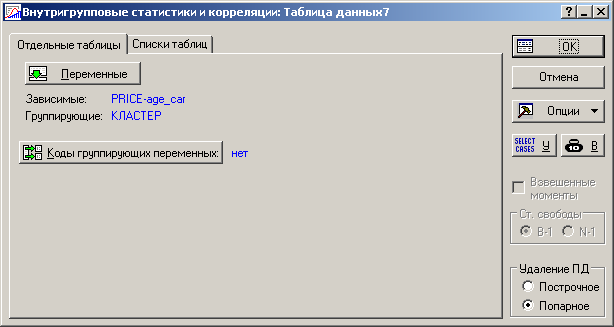
\includegraphics[width=12cm]
  {inc/cars_my/3.11.PNG}

  \caption{Окно <<Внутригрупповые статистики и корреляции>>}
  \label{fig:3_11}
\end{figure}

\begin{figure}[!ph]
  \centering
  \begin{minipage}{0.49\textwidth}
    \centering

    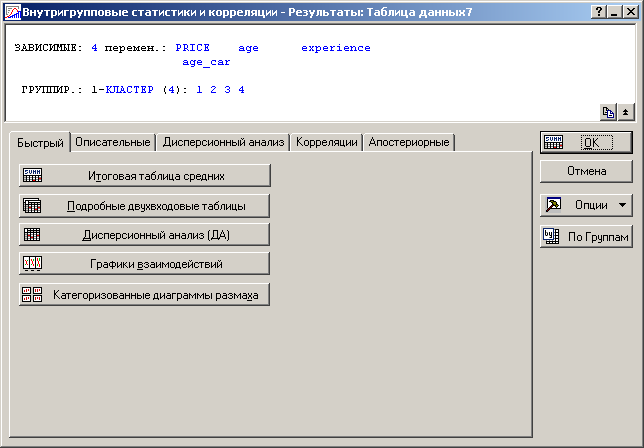
\includegraphics[height=6cm]
    {inc/cars_my/3.12.PNG}

    \caption{Окно <<Внутригрупповые статистики и корреляции>>}
    \label{fig:3_12}
  \end{minipage}
  \begin{minipage}{0.49\textwidth}
    \centering

    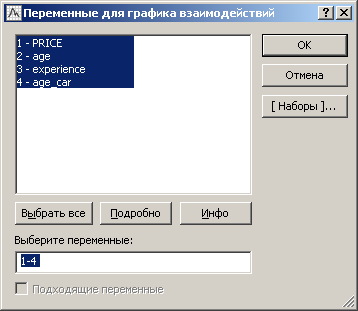
\includegraphics[height=6cm]
    {inc/cars_my/3.13.PNG}

    \caption{Окно <<Переменные для графика взаимодействий>>}
    \label{fig:3_13}
  \end{minipage}
\end{figure}

\begin{figure}[!ph]
  \centering

  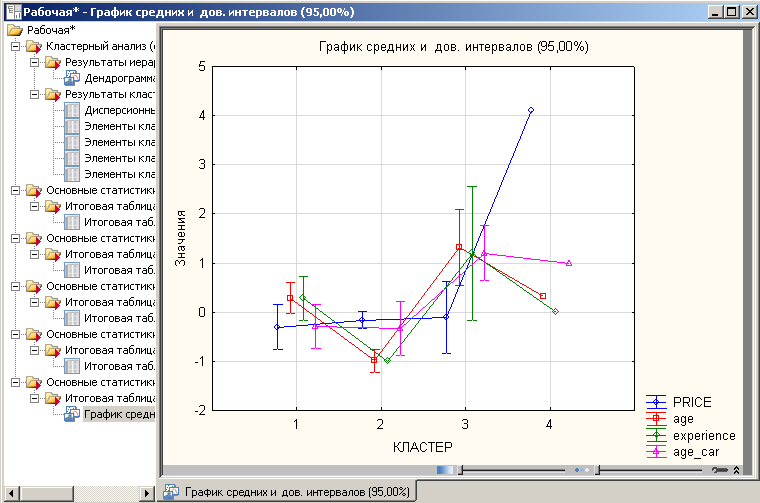
\includegraphics[height=8.2cm]
  {inc/cars_my/3.14.PNG}

  \caption{График средних и дов. интервалов (95.00\%)}
  \label{fig:3_14}
\end{figure}

\newpage

\begin{center}
  \textbf{Вариант 5}
\end{center}

Удаляю папку <<Statistica 10 RUS>>.

Запускаю Ststatistica\_10\_ru\_portable.exe.

Главная > Открыть > <<Country data for vars.xls>> > Открыть \\
> Импортировать выбранные лист в Таблицу данных > Var5 > OK \\
> Имена переменных из первой строки>Имена наблюдений из первого столбца > OK

Результат смотри на рисунке~\ref{fig:var5__1_1}.

\begin{figure}[!h]
  \centering

  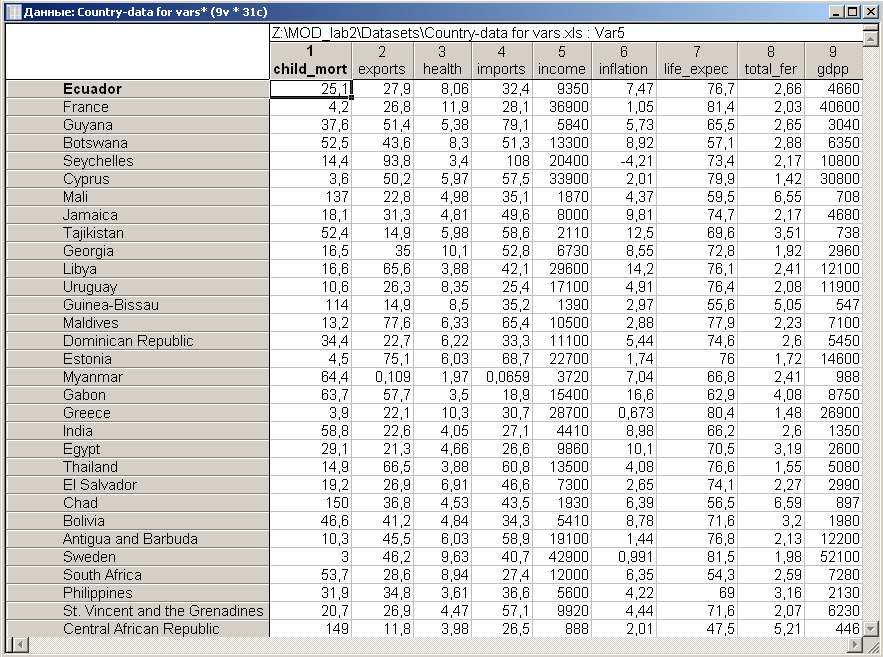
\includegraphics[height=12cm]
  {inc/cars_my/var5__1_1.PNG}

  \caption{Открыли cars\_my.xls в Statistica 10}

  \label{fig:var5__1_1}
\end{figure}

\begin{center}
  \textbf{Масштаб измерений}
\end{center}

Данные > Стандартизировать > Переменные > Выбрать все > OK > OK

Результат смотри на рисунке~\ref{fig:var5__1_2}.

\begin{figure}[!h]
  \centering

  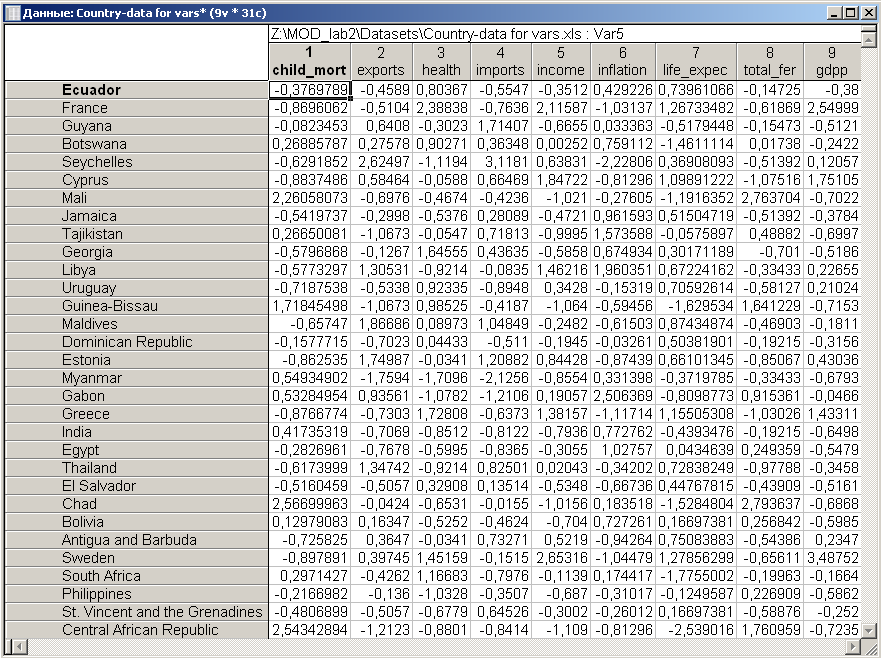
\includegraphics[height=12cm]
  {inc/cars_my/var5__1_2.PNG}

  \caption{Данные}

  \label{fig:var5__1_2}
\end{figure}

Кружок > Сохранить как... > Country\_data\_var5\_standartiz.sta > Сохранить

\newpage

\begin{center}
  \textbf{Шаг 1. Иерархическая классификация}
\end{center}

Анализ > Многомерный анализ > Кластерный анализ > Иерархическая классификация > OK \\
> Дополнительно > Переменные > Выбрать все > OK \\
> Объекты > Наблюдения (строки) \\
> Правило объединения > Метод полной связи \\
> Мера близости > Евклидово расстояние \\
> OK > Дополнительно > Вертикальная дендрограмма

Результаты смотри на рисунках~\ref{fig:var5__1_3}, \ref{fig:var5__1_4}, \ref{fig:var5__1_5}.

\begin{figure}[!h]
  \centering
  \begin{minipage}{0.49\textwidth}
    \centering

    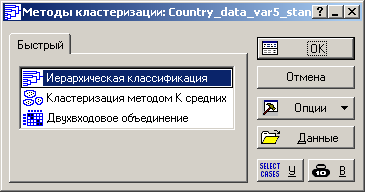
\includegraphics[width=0.99\textwidth]
    {inc/cars_my/var5__1_3.PNG}

    \caption{Окно <<Методы кластеризации>>}
    \label{fig:var5__1_3}
  \end{minipage}
  \begin{minipage}{0.49\textwidth}
    \centering

    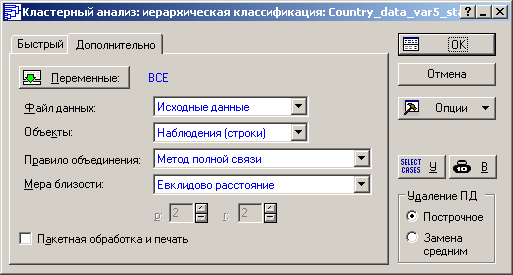
\includegraphics[width=0.99\textwidth]
    {inc/cars_my/var5__1_4.PNG}

    \caption{Окно <<Кластерный анализ>>}
    \label{fig:var5__1_4}
  \end{minipage}
\end{figure}

\begin{figure}[!h]
  \centering

  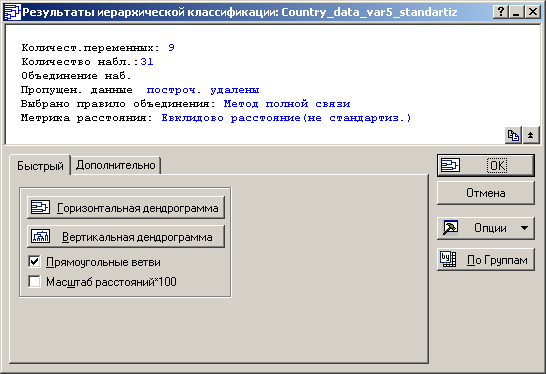
\includegraphics[height=10cm]
  {inc/cars_my/var5__1_5.PNG}

  \caption{Окно <<Результаты иерархической классификации>>}
  \label{fig:var5__1_5}
\end{figure}

\newpage

Результат смотри на рисунке~\ref{fig:var5__1_6}.

\begin{figure}[!h]
  \centering

  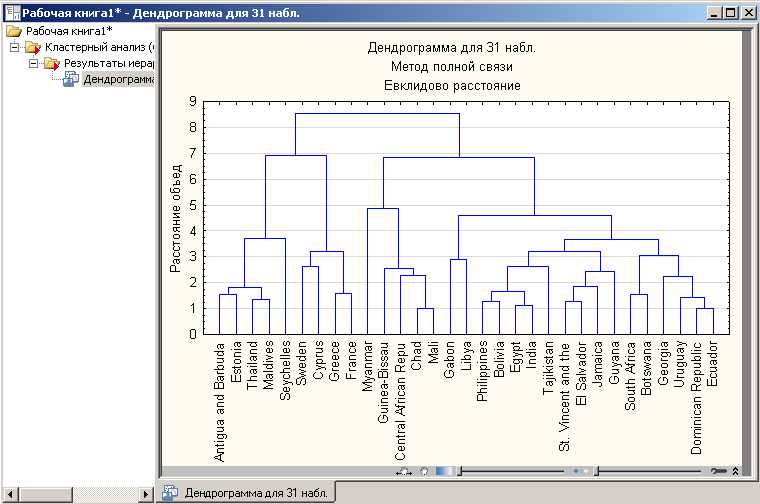
\includegraphics[width=17cm]
  {inc/cars_my/var5__1_6.PNG}

  \caption{Дендрограмма для 31 набл.}
  \label{fig:var5__1_6}
\end{figure}

\newpage

\begin{center}
  \textbf{Шаг 2. Кластеризация методом К средних}
\end{center}

Результата иерархической классификации: Country-data for vars > Отмена > Отмена \\
> Кластеризация методом К средних > OK \\
> Дополнительно \\
> Переменные > Выбрать все > OK \\
> Объекты > Наблюдения (строки) \\
> Число кластеров > 7 \\
> OK > Дополнительно > Дисперсионный анализ

Результаты смотри на рисунках~\ref{fig:var5__2_1}, \ref{fig:var5__2_2}, \ref{fig:var5__2_3}.

\begin{figure}[!h]
  \centering
  \begin{minipage}{0.49\textwidth}
    \centering

    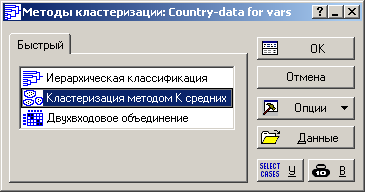
\includegraphics[width=0.99\textwidth]
    {inc/cars_my/var5__2_1.PNG}

    \caption{Окно <<Методы кластеризации>>}
    \label{fig:var5__2_1}
  \end{minipage}
  \begin{minipage}{0.49\textwidth}
    \centering

    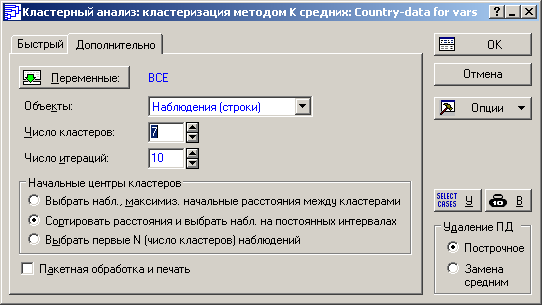
\includegraphics[width=0.99\textwidth]
    {inc/cars_my/var5__2_2.PNG}

    \caption{Окно <<Кластерный анализ>>}
    \label{fig:var5__2_2}
  \end{minipage}
\end{figure}

\begin{figure}[!h]
  \centering

  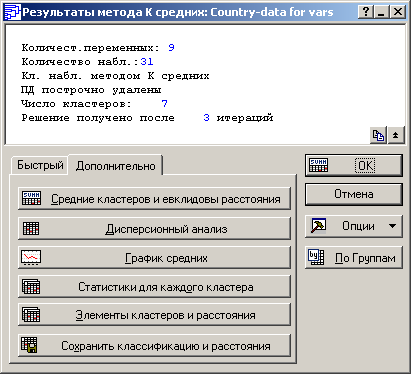
\includegraphics[height=10cm]
  {inc/cars_my/var5__2_3.PNG}

  \caption{Дисперсионный анализ}
  \label{fig:var5__2_3}
\end{figure}

\newpage

Результаты смотри на рисунке~\ref{fig:var5__2_4}.

\begin{figure}[!h]
  \centering

  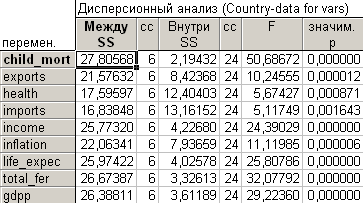
\includegraphics[height=8cm]
  {inc/cars_my/var5__2_4.PNG}

  \caption{Дисперсионный анализ}
  \label{fig:var5__2_4}
\end{figure}

Результаты метода К средних: Country-data for vars > Дополнительно > Элементы кластеров и расстояния

Данные первого кластера смотри на рисунке~\ref{fig:var5__2_5}.

Данные второго кластера смотри на рисунке~\ref{fig:var5__2_6}.

\begin{figure}[!h]
  \centering
  \begin{minipage}{0.49\textwidth}
    \centering

    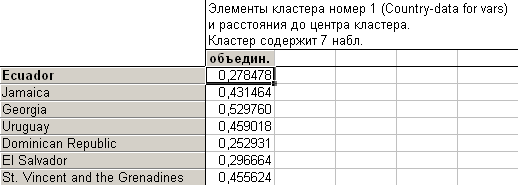
\includegraphics[width=0.99\textwidth]
    {inc/cars_my/var5__2_5.PNG}

    \caption{Первый кластер}
    \label{fig:var5__2_5}
  \end{minipage}
  \begin{minipage}{0.49\textwidth}
    \centering

    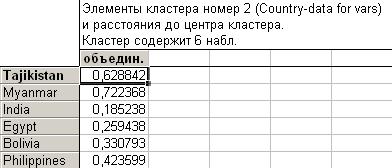
\includegraphics[width=0.99\textwidth]
    {inc/cars_my/var5__2_6.PNG}

    \caption{Второй кластер}
    \label{fig:var5__2_6}
  \end{minipage}
\end{figure}

Данные третьего кластера смотри на рисунке~\ref{fig:var5__2_7}.

Данные четвертого кластера смотри на рисунке~\ref{fig:var5__2_8}.

\begin{figure}[!h]
  \centering
  \begin{minipage}{0.49\textwidth}
    \centering

    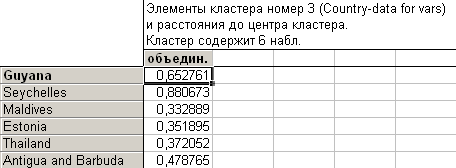
\includegraphics[width=0.99\textwidth]
    {inc/cars_my/var5__2_7.PNG}

    \caption{Третий кластер}
    \label{fig:var5__2_7}
  \end{minipage}
  \begin{minipage}{0.49\textwidth}
    \centering

    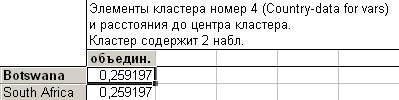
\includegraphics[width=0.99\textwidth]
    {inc/cars_my/var5__2_8.PNG}

    \caption{Четвертый кластер}
    \label{fig:var5__2_8}
  \end{minipage}
\end{figure}

\newpage

Данные пятого кластера смотри на рисунке~\ref{fig:var5__2_9}.

Данные шестого кластера смотри на рисунке~\ref{fig:var5__2_10}.

\begin{figure}[!h]
  \centering
  \begin{minipage}{0.49\textwidth}
    \centering

    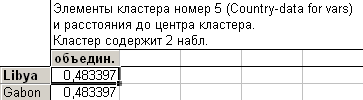
\includegraphics[width=0.99\textwidth]
    {inc/cars_my/var5__2_9.PNG}

    \caption{Пятый кластер}
    \label{fig:var5__2_9}
  \end{minipage}
  \begin{minipage}{0.49\textwidth}
    \centering

    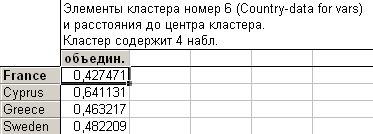
\includegraphics[width=0.99\textwidth]
    {inc/cars_my/var5__2_10.PNG}

    \caption{Шестой кластер}
    \label{fig:var5__2_10}
  \end{minipage}
\end{figure}

Данные седьмого кластера смотри на рисунке~\ref{fig:var5__2_11}.

\begin{figure}[!h]
  \centering

  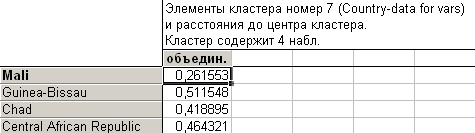
\includegraphics[width=16cm]
  {inc/cars_my/var5__2_11.PNG}

  \caption{Седьмой кластер}
  \label{fig:var5__2_11}
\end{figure}

\newpage

\begin{center}
  \textbf{Шаг 3. Кластеризация методом К средних}
\end{center}

Результаты метода К средних: cars\_my\_standartiz > Дополнительно > Сохранить классификацию и расстояние > Выбрать все > OK

Результаты смотри на рисунках~\ref{fig:var5__3_1}, \ref{fig:var5__3_2}, \ref{fig:var5__3_3}.

\begin{figure}[!h]
  \centering
  \begin{minipage}{0.49\textwidth}
    \centering

    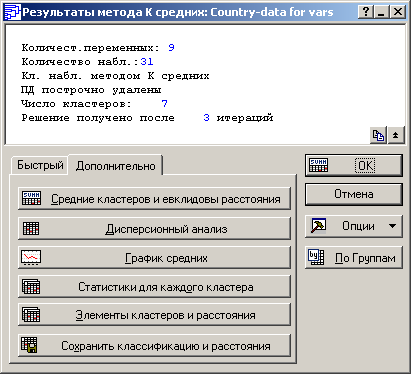
\includegraphics[width=0.99\textwidth]
    {inc/cars_my/var5__3_1.PNG}

    \caption{Окно <<Основные статистики и таблицы>>}
    \label{fig:var5__3_1}
  \end{minipage}
  \begin{minipage}{0.49\textwidth}
    \centering

    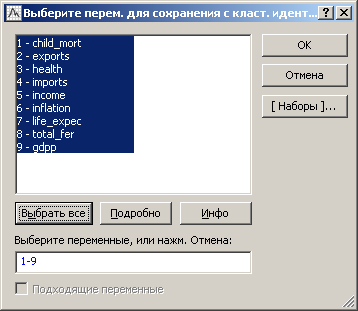
\includegraphics[width=0.99\textwidth]
    {inc/cars_my/var5__3_2.PNG}

    \caption{Окно <<Внутригрупповые статистики и корреляции>>}
    \label{fig:var5__3_2}
  \end{minipage}
\end{figure}

\begin{figure}[!h]
  \centering

  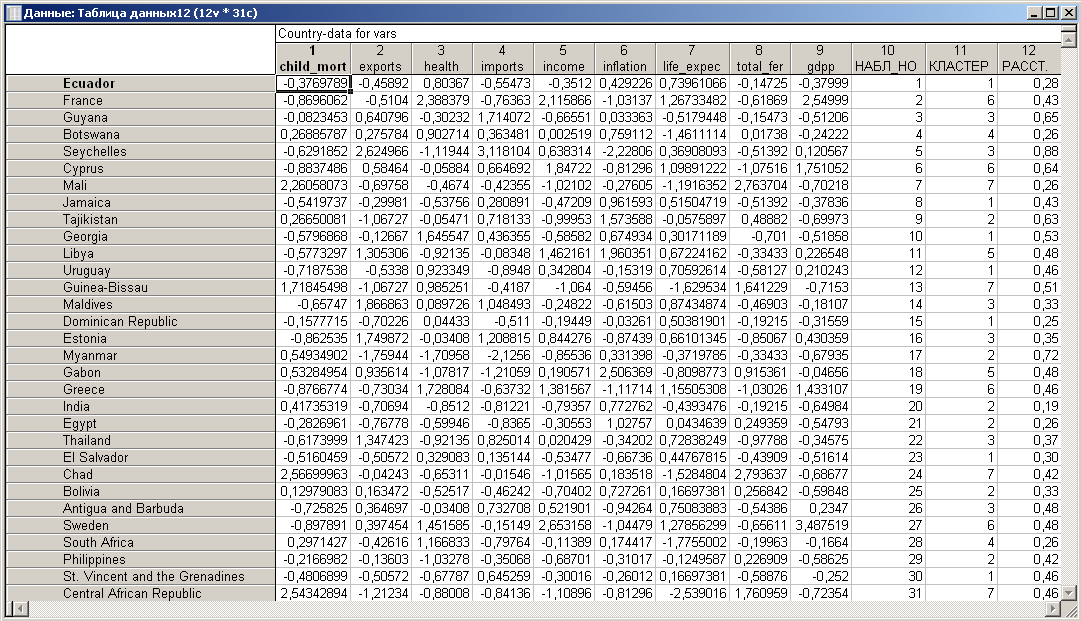
\includegraphics[width=0.99\textwidth]
  {inc/cars_my/var5__3_3.PNG}

  \caption{Окно <<Выберите зависимые и группирующие переменные>>}
  \label{fig:var5__3_3}
\end{figure}

\newpage

Анализ > Основные статистики и таблицы\\
> Группировка и однофакторный ДА > OK\\
> Переменные > 1-child\_mort > 11-КЛАСТЕР > OK > OK\\
> Описательные\\
> Статистики > Минимум и максимум\\
> Итоговая таблица средних

Результаты на рисунках~\ref{fig:var5__3_4}, \ref{fig:var5__3_5}, \ref{fig:var5__3_6}, \ref{fig:var5__3_7}.

\begin{figure}[!h]
  \centering
  \begin{minipage}{0.49\textwidth}
    \centering

    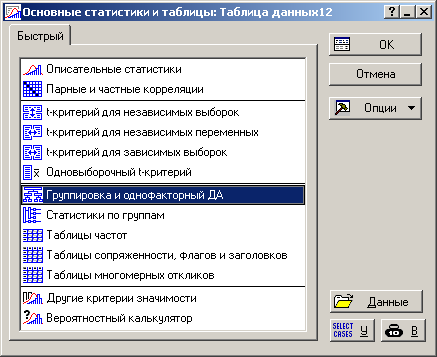
\includegraphics[width=0.99\textwidth]
    {inc/cars_my/var5__3_4.PNG}

    \caption{Окно <<Основные статистики и таблицы>>}
    \label{fig:var5__3_4}
  \end{minipage}
  \begin{minipage}{0.49\textwidth}
    \centering

    \includegraphics[width=0.99\textwidth]
    {inc/cars_my/var5__3_5.PNG}

    \caption{Окно <<Выберите зависимые и группирующие переменные>>}
    \label{fig:var5__3_5}
  \end{minipage}
\end{figure}

\begin{figure}[!h]
  \centering
  \begin{minipage}{0.49\textwidth}
    \centering

    \includegraphics[width=0.99\textwidth]
    {inc/cars_my/var5__3_6.PNG}

    \caption{Окно <<Внутригрупповые статистики и корреляции>>}
    \label{fig:var5__3_6}
  \end{minipage}
  \begin{minipage}{0.49\textwidth}
    \centering

    \includegraphics[width=0.99\textwidth]
    {inc/cars_my/var5__3_7.PNG}

    \caption{child\_mort}
    \label{fig:var5__3_7}
  \end{minipage}
\end{figure}

Анализ > Основные статистики и таблицы > Новый\\
> Группировка и однофакторный ДА > OK\\
> Переменные > 2-exports > 11-КЛАСТЕР > OK > OK\\
> Описательные\\
> Статистики > Минимум и максимум\\
> Итоговая таблица средних

Результат на рисунке~\ref{fig:var5__3_8}.

\newpage

Анализ > Основные статистики и таблицы > Новый\\
> Группировка и однофакторный ДА > OK\\
> Переменные > 3-health > 11-КЛАСТЕР > OK > OK\\
> Описательные\\
> Статистики > Минимум и максимум\\
> Итоговая таблица средних

Результат на рисунке~\ref{fig:var5__3_9}.

\begin{figure}[!h]
  \centering
  \begin{minipage}{0.49\textwidth}
    \centering

    \includegraphics[width=0.99\textwidth]
    {inc/cars_my/var5__3_8.PNG}

    \caption{exports}
    \label{fig:var5__3_8}
  \end{minipage}
  \begin{minipage}{0.49\textwidth}
    \centering

    \includegraphics[width=0.99\textwidth]
    {inc/cars_my/var5__3_9.PNG}

    \caption{health}
    \label{fig:var5__3_9}
  \end{minipage}
\end{figure}

Анализ > Основные статистики и таблицы > Новый\\
> Группировка и однофакторный ДА > OK\\
> Переменные > 4-imports > 11-КЛАСТЕР > OK > OK\\
> Описательные\\
> Статистики > Минимум и максимум\\
> Итоговая таблица средних

Результат на рисунке~\ref{fig:var5__3_10}.

Анализ > Основные статистики и таблицы > Новый\\
> Группировка и однофакторный ДА > OK\\
> Переменные > 5-income > 11-КЛАСТЕР > OK > OK\\
> Описательные\\
> Статистики > Минимум и максимум\\
> Итоговая таблица средних

Результат на рисунке~\ref{fig:var5__3_11}.

\begin{figure}[!h]
  \centering
  \begin{minipage}{0.49\textwidth}
    \centering

    \includegraphics[width=0.99\textwidth]
    {inc/cars_my/var5__3_10.PNG}

    \caption{imports}
    \label{fig:var5__3_10}
  \end{minipage}
  \begin{minipage}{0.49\textwidth}
    \centering

    \includegraphics[width=0.99\textwidth]
    {inc/cars_my/var5__3_11.PNG}

    \caption{income}
    \label{fig:var5__3_11}
  \end{minipage}
\end{figure}

\newpage

Анализ > Основные статистики и таблицы > Новый\\
> Группировка и однофакторный ДА > OK\\
> Переменные > 6-inflation > 11-КЛАСТЕР > OK > OK\\
> Описательные > Статистики > Минимум и максимум\\
> Итоговая таблица средних. Результат на рисунке~\ref{fig:var5__3_12}.

Анализ > Основные статистики и таблицы > Новый\\
> Группировка и однофакторный ДА > OK\\
> Переменные > 7-life\_expec > 11-КЛАСТЕР > OK > OK\\
> Описательные > Статистики > Минимум и максимум\\
> Итоговая таблица средних. Результат на рисунке~\ref{fig:var5__3_13}.

\begin{figure}[!h]
  \centering
  \begin{minipage}{0.49\textwidth}
    \centering

    \includegraphics[width=0.99\textwidth]
    {inc/cars_my/var5__3_12.PNG}

    \caption{inflation}
    \label{fig:var5__3_12}
  \end{minipage}
  \begin{minipage}{0.49\textwidth}
    \centering

    \includegraphics[width=0.99\textwidth]
    {inc/cars_my/var5__3_13.PNG}

    \caption{life\_expec}
    \label{fig:var5__3_13}
  \end{minipage}
\end{figure}

Анализ > Основные статистики и таблицы > Новый\\
> Группировка и однофакторный ДА > OK\\
> Переменные > 8-total\_fer > 11-КЛАСТЕР > OK > OK\\
> Описательные > Статистики > Минимум и максимум\\
> Итоговая таблица средних. Результат на рисунке~\ref{fig:var5__3_14}.

Анализ > Основные статистики и таблицы > Новый\\
> Группировка и однофакторный ДА > OK\\
> Переменные > 9-gdpp > 11-КЛАСТЕР > OK > OK\\
> Описательные > Статистики > Минимум и максимум\\
> Итоговая таблица средних. Результат на рисунке~\ref{fig:var5__3_15}.

\begin{figure}[!h]
  \centering
  \begin{minipage}{0.49\textwidth}
    \centering

    \includegraphics[width=0.99\textwidth]
    {inc/cars_my/var5__3_14.PNG}

    \caption{total\_fer}
    \label{fig:var5__3_14}
  \end{minipage}
  \begin{minipage}{0.49\textwidth}
    \centering

    \includegraphics[width=0.99\textwidth]
    {inc/cars_my/var5__3_15.PNG}

    \caption{gdpp}
    \label{fig:var5__3_15}
  \end{minipage}
\end{figure}

\newpage

Анализ > Основные статистики и таблицы > Новый\\
> Группировка и однофакторный ДА > OK\\
> Переменные > (1-child\_mort, 2-exports, 3-health, 4-imports, 5-income,
7-inflation, 7-life\_expec, 8-total\_fer, 9-gdpp) > 11-КЛАСТЕР > OK > OK\\
> Описательные > Статистики > Минимум и максимум\\
> Итоговая таблица средних

Результат на рисунке~\ref{fig:var5__3_16}, \ref{fig:var5__3_17}, \ref{fig:var5__3_18}, \ref{fig:var5__3_19}, \ref{fig:var5__3_20}, \ref{fig:var5__3_21}.

\begin{figure}[!h]
  \centering
  \begin{minipage}{0.49\textwidth}
    \centering

    \includegraphics[width=0.99\textwidth]
    {inc/cars_my/var5__3_16.PNG}

    \caption{Окно <<Внутригрупповые статистики и корреляции>>}
    \label{fig:var5__3_16}
  \end{minipage}
  \begin{minipage}{0.49\textwidth}
    \centering

    \includegraphics[width=0.99\textwidth]
    {inc/cars_my/var5__3_17.PNG}

    \caption{Окно <<Переменные для графика взаимодействий>>}
    \label{fig:var5__3_17}
  \end{minipage}
\end{figure}

\begin{figure}[!h]
  \centering

  \includegraphics[width=0.99\textwidth]
  {inc/cars_my/var5__3_18.PNG}

  \caption{Окно <<Внутригрупповые статистики и корреляции>>}
  \label{fig:var5__3_18}
\end{figure}

\begin{figure}[!ph]
  \centering
  \begin{minipage}{0.49\textwidth}
    \centering

    \includegraphics[width=0.99\textwidth]
    {inc/cars_my/var5__3_19.PNG}

    \caption{Окно <<Внутригрупповые статистики и корреляции>>}
    \label{fig:var5__3_19}
  \end{minipage}
  \begin{minipage}{0.49\textwidth}
    \centering

    \includegraphics[width=0.99\textwidth]
    {inc/cars_my/var5__3_20.PNG}

    \caption{Окно <<Переменные для графика взаимодействий>>}
    \label{fig:var5__3_20}
  \end{minipage}
\end{figure}

\begin{figure}[!ph]
  \centering

  \includegraphics[height=12cm]
  {inc/cars_my/var5__3_21.PNG}

  \caption{График средних и дов. интервалов (95.00\%)}
  \label{fig:var5__3_21}
\end{figure}
